\documentclass{article}
\usepackage{graphicx}
\usepackage{amsmath}
\usepackage{geometry}
\usepackage{lipsum}
\usepackage{listings}
\usepackage{xcolor}
\usepackage{setspace}

\lstset{
    language=Python,
    basicstyle=\small\ttfamily,
    keywordstyle=\color{blue},
    stringstyle=\color{green!60!black},
    commentstyle=\color{gray}\itshape,
    showstringspaces=false,
    breaklines=true,
    numbers=left,
    numberstyle=\tiny,
    frame=single,
    backgroundcolor=\color{gray!10},
    captionpos=b 
}

\geometry{
    a4paper,
    left=25mm,
    right=25mm,
    top=20mm,
    bottom=20mm,
}

\begin{document}
\title{Double Pendulum using Euler-Lagrangian Equations}
\author{Sujal Bajracharya, Yajjyu Tuladhar}
\date{June 2024}

\begin{titlepage}
    \centering
    \vspace*{1.5cm}

    {\huge\bfseries Double Pendulum using Euler-Lagrangian Equations\par}
     \vspace{2.5cm}
     
\includegraphics[width=0.3\textwidth]{KU-Logo.png}\par
    \vspace{0.5cm}
    {\Large \textbf{Kathmandu University \\ Dhulikhel, Kavre}}\\
    \vspace{2.5cm}
    \begin{center}
        
        \vspace{1cm}
        
        {\large \textbf{Submitted by:}} \\
        Sujal Bajracharya (4) \\
        Yajjyu Tuladhar (27) \\
        Department of Computer Science and Engineering \\
        Kathmandu University
    
        \vspace{1.5cm}
        {\large \textbf{Submitted to:}}\\
        Mr.\ Harish Chandra Bhandari \\
        Department of Mathematics \\
        Kathmandu University \\

        \vspace{1.5cm}
        {\large \textbf{Submition Date: }}\\
        \today
    \end{center}

    

    
    \vspace{1cm}
\end{titlepage}

\newpage
\tableofcontents
\vspace{1cm}
\listoffigures

\newpage
\section{Objectives}
\begin{enumerate}
    \item Deriving the equations for the double pendulum using the Lagrangian Method.
    \item Creating a simulation of the double pendulum.
    \item Learning latex.
\end{enumerate}
\newpage
\section{Introduction}

\subsection{Simple Pendulum}
A simple pendulum consists of a mass, referred to as a bob, attached to the end of a rod of fixed length, which pivots from a fixed point. When displaced from its equilibrium position and released, the pendulum oscillates back and forth under the influence of gravity.
\\
\begin{figure}[h]
        \centering
        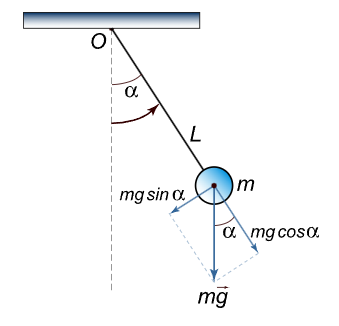
\includegraphics[width=0.45\linewidth]{single.png}
        \caption{Single Pendulum}
\end{figure}\\
The motion of a simple pendulum can be described by a second-order differential equation derived from Newton’s second law. Consider a pendulum of length \( l \) and bob mass \( m \). When the pendulum is displaced by an angle \( \theta \) from the vertical, the restoring force due to gravity is \( -mg \sin \theta \).

Using the small-angle approximation (\(\sin \theta \approx \theta\) for small angles), the torque \( \tau \) about the pivot point is given by:
\[
\tau = -mgl\theta
\]

According to Newton’s second law for rotational motion, the torque is equal to the moment of inertia \( I \) times the angular acceleration \( \alpha \):
\[
\tau = I \alpha
\]

For a pendulum, the moment of inertia \( I \) about the pivot point is:
\[
I = ml^2
\]

Substituting \( \tau \) and \( I \) into Newton's second law for rotational motion, we get:
\[
-mgl\theta = ml^2 \frac{d^2 \theta}{dt^2}
\]

Simplifying this equation by dividing both sides by \( ml^2 \), we obtain the second-order differential equation:
\[
\frac{d^2 \theta}{dt^2} + \frac{g}{l} \theta = 0
\]

This is a simple harmonic oscillator equation with angular frequency \( \omega \):
\[
\omega = \sqrt{\frac{g}{l}}
\]

The general solution to this differential equation is:
\[
\theta(t) = \theta_0 \cos\left( \sqrt{\frac{g}{l}} t + \phi \right)
\]

where \( \theta_0 \) is the maximum angular displacement (amplitude) and \( \phi \) is the phase constant determined by the initial conditions.


\newpage
\subsection{Double Pendulum}

The double pendulum, is an iconic example of \textbf{chaotic motion}, captivates our engineering imagination with its unpredictable behaviour. It is a system comprising two single pendulums in tandem resulting in a system with two degrees of freedom, leading to highly complex dynamics, especially for larger angles of displacement. 

The motion of the double pendulum is governed by a set of coupled \textbf{nonlinear differential equations}. Unlike the simple pendulum, the double pendulum exhibits sensitive dependence on initial conditions, making it a classic example of a chaotic system in classical mechanics.
\\
\begin{figure}[h]
        \centering
        \includegraphics[width=0.5\linewidth]{WhatsApp Image 2024-06-16 at 14.49.55_9247e1e2.jpg}
        \caption{Double Pendulum}
\end{figure}\\
Consider a double pendulum with lengths \( l_1 \) and \( l_2 \), and masses \( m_1 \) and \( m_2 \), where \( \theta_1 \) and \( \theta_2 \) are the angles of the first and second pendulums from the vertical, respectively. \\ 
After differentiating and simplifying, the equations of motion for \(\theta_1\) and \(\theta_2\) are:

\[
\begin{aligned}
\alpha_1 &= \frac{-g (2 m_1 + m_2) \sin(\theta_1) - m_2 g \sin(\theta_1 - 2 \theta_2) - 2 \sin(\theta_1 - \theta_2) m_2 \left( \dot{\theta}_2^2 L_2 + \dot{\theta}_1^2 L_1 \cos(\theta_1 - \theta_2) \right)}{L_1 \left( 2 m_1 + m_2 - m_2 \cos(2 \theta_1 - 2 \theta_2) \right)},
\end{aligned}
\]

\[
\begin{aligned}
\alpha_2 &= \frac{2 \sin(\theta_1 - \theta_2) \left( \dot{\theta}_1^2 L_1 (m_1 + m_2) + g (m_1 + m_2) \cos(\theta_1) + \dot{\theta}_2^2 L_2 m_2 \cos(\theta_1 - \theta_2) \right)}{L_2 \left( 2 m_1 + m_2 - m_2 \cos(2 \theta_1 - 2 \theta_2) \right)}.
\end{aligned}
\]
\\
These equations describe the highly complex and often chaotic motion of the double pendulum, showcasing its sensitive dependence on initial conditions.
 

\subsection{Lagrangian Mechanics in Double Pendulum}
The Lagrangian, denoted as L, serves as the foundation of the Lagrangian approach. It is defined as the difference between the kinetic energy (T) and potential energy (V) of the system. This seemingly simple expression encapsulates the essence of the system's dynamics.\\

The Lagrangian (L) for the double pendulum is defined as:
\[ L=T-V\]

Lagrangian mechanics is often a superior choice for analysing complex mechanical systems like the double pendulum for several reasons:

\begin{itemize}
  \item \textbf{Generalised Coordinates}: It allows us to use generalised coordinates (\( \theta_1 \) and \(\theta_2\)) that describe the system's configuration. This simplifies the analysis by reducing the number of variables compared to Cartesian coordinates.
    \\ 
  \item \textbf{No Need for Constraints}: In the case of the double pendulum, there is a constraint due to the fixed length of the rods, and Lagrangian mechanics can handle this constraint without the need for additional equations.
  \item \textbf{Derivation of Equations}: By applying Lagrange's equations, we obtain a set of second-order differential equations that govern the system's motion directly. 
\end{itemize}

The use of small angle approximation cannot be applied to a double pendulum because the system is highly nonlinear and chaotic. Below are a few reasons:

\begin{enumerate}
    \item \textbf{Nonlinearity}: In a simple pendulum, the restoring force is directly proportional to the angle the pendulum makes with the vertical. This allows us to use a small angle approximation () to simplify the equations of motion. However, in a double pendulum, the restoring forces are not linearly proportional to the angles, which leads to highly nonlinear equations of motion. 
    \item \textbf{Chaos}: A double pendulum is a chaotic system, meaning it is highly sensitive to initial conditions. Even small changes in the initial positions or velocities of the pendulum can lead to dramatically different trajectories. This chaotic behaviour is a result of the complex, nonlinear interactions between the two pendulum arms.
    \item \textbf{Complex Dynamics}: The motion of a double pendulum involves multiple coupled differential equations that are difficult to solve analytically. These equations cannot be easily reduced to a linear approximation like in the case of a simple pendulum.
\end{enumerate}


\newpage
\section{Derivation of Formulas}
The double pendulum consists of two point masses, \(m_1\) and \(m_2\), attached to two rigid rods of lengths \(l_1\) and \(l_2\), respectively.\ \(\theta_1\) and \(\theta_2\) are angles made by the respective rods with normal. The goal is to derive the equations of motion using the Lagrangian method.
\subsection{Coordinates}

The positions of the masses are given by:
\[
\begin{aligned}
    x_1 &= l_1 \sin \theta_1, \\
    y_1 &= -l_1 \cos \theta_1, \\
    x_2 &= l_1 \sin \theta_1 + l_2 \sin \theta_2, \\
    y_2 &= -l_1 \cos \theta_1 - l_2 \cos \theta_2.
\end{aligned}
\]

Calculating the derivatives, we get:
\[
\begin{aligned}
    \dot{x}_1 &= l_1 \dot{\theta}_1 \cos \theta_1, \\
    \dot{y}_1 &= l_1 \dot{\theta}_1 \sin \theta_1, \\
    \dot{x}_2 &= l_1 \dot{\theta}_1 \cos \theta_1 + l_2 \dot{\theta}_2 \cos \theta_2, \\
    \dot{y}_2 &= l_1 \dot{\theta}_1 \sin \theta_1 + l_2 \dot{\theta}_2 \sin \theta_2.
\end{aligned}
\]
These will be needed for further calculation of Kinetic energy, Potential energy and Lagrangian.
\\
\subsection{Kinetic Energy}
The kinetic energy \(T\) of the system is:
\[
T = \frac{1}{2} m_1 (\dot{x}_1^2 + \dot{y}_1^2) + \frac{1}{2} m_2 (\dot{x}_2^2 + \dot{y}_2^2).
\]

Thus,
\[
\begin{aligned}
    T &= \frac{1}{2} m_1 (l_1^2 \dot{\theta}_1^2) + \frac{1}{2} m_2 (l_1^2 \dot{\theta}_1^2 + l_2^2 \dot{\theta}_2^2 + 2 l_1 l_2 \dot{\theta}_1 \dot{\theta}_2 \cos(\theta_1 - \theta_2)).
\end{aligned}
\]
\\
\subsection{Potential Energy}

The potential energy \(V\) of the system is:
\[
V = -m_1 g y_1 - m_2 g y_2 = m_1 g l_1 \cos \theta_1 + m_2 g (l_1 \cos \theta_1 + l_2 \cos \theta_2).
\]
\\
\subsection{Lagrangian Equations}
The Lagrangian \(L\) is given by:
\[L = T - V \]
\[L = \frac{1}{2} m_1 l_1^2 \dot{\theta}_1^2 + \frac{1}{2} m_2 \left(l_1^2 \dot{\theta}_1^2 + l_2^2 \dot{\theta}_2^2 + 2 l_1 l_2 \dot{\theta}_1 \dot{\theta}_2 \cos(\theta_1 - \theta_2)\right) - m_1 g l_1 \cos \theta_1 - m_2 g (l_1 \cos \theta_1 + l_2 \cos \theta_2).
\]
\\
Using the Euler-Lagrange equations:
\[
\frac{d}{dt} \left( \frac{\partial L}{\partial \dot{\theta}_i} \right) - \frac{\partial L}{\partial \theta_i} = 0,
\]
The Euler-Lagrange equations for generalized coordinates \(\theta_1\) and \(\theta_2\) are:
\begin{align}
\frac{d}{dt} \left( \frac{\partial \mathcal{L}}{\partial \dot{\theta}_1} \right) - \frac{\partial \mathcal{L}}{\partial \theta_1} &= 0 \label{eq:euler-lagrange1} \\
\frac{d}{dt} \left( \frac{\partial \mathcal{L}}{\partial \dot{\theta}_2} \right) - \frac{\partial \mathcal{L}}{\partial \theta_2} &= 0 \label{eq:euler-lagrange2}
\end{align}
\\
First, compute the partial derivatives for \(\theta_1\):
\[\frac{\partial \mathcal{L}}{\partial \dot{\theta}_1} = m_1 l_1^2 \dot{\theta}_1 + m_2 \left( l_1^2 \dot{\theta}_1 + l_1 l_2 \dot{\theta}_2 \cos(\theta_1 - \theta_2) \right)\]

\[\frac{d}{dt} \left( \frac{\partial \mathcal{L}}{\partial \dot{\theta}_1} \right) = m_1 l_1^2 \ddot{\theta}_1 + m_2 \left( l_1^2 \ddot{\theta}_1 + l_1 l_2 \left( \ddot{\theta}_2 \cos(\theta_1 - \theta_2) - \dot{\theta}_1 \dot{\theta}_2 \sin(\theta_1 - \theta_2) \right) \right)\]

\[\frac{\partial \mathcal{L}}{\partial \theta_1} = -m_1 g l_1 \sin \theta_1 - m_2 g l_1 \sin \theta_1 - m_2 l_1 l_2 \dot{\theta}_1 \dot{\theta}_2 \sin(\theta_1 - \theta_2)\]
\\
Similarly, for \(\theta_2\):
\[
\frac{\partial \mathcal{L}}{\partial \dot{\theta}_2} = m_2 l_2^2 \dot{\theta}_2 + m_2 l_1 l_2 \dot{\theta}_1 \cos(\theta_1 - \theta_2)
\]

\[
\frac{d}{dt} \left( \frac{\partial \mathcal{L}}{\partial \dot{\theta}_2} \right) = m_2 l_2^2 \ddot{\theta}_2 + m_2 l_1 l_2 \left( \ddot{\theta}_1 \cos(\theta_1 - \theta_2) - \dot{\theta}_1 \dot{\theta}_2 \sin(\theta_1 - \theta_2) \right)
\]

\[
\frac{\partial \mathcal{L}}{\partial \theta_2} = -m_2 g l_2 \sin \theta_2 + m_2 l_1 l_2 \dot{\theta}_1 \dot{\theta}_2 \sin(\theta_1 - \theta_2)
\]

\subsection*{Euler-Lagrangian Equations}
Now, substituting everything in \eqref{eq:euler-lagrange1} and \eqref{eq:euler-lagrange2}.

\begin{align}
(m_1 + m_2) l_1 \ddot{\theta}_1 + m_2 l_2 \ddot{\theta}_2 \cos(\theta_1 - \theta_2) + m_2 l_2 \dot{\theta}_2^2 \sin(\theta_1 - \theta_2) &= - (m_1 + m_2) g \sin \theta_1 \label{eq:equation3} \\
m_2 l_2 \ddot{\theta}_2 + m_2 l_1 \ddot{\theta}_1 \cos(\theta_1 - \theta_2) - m_2 l_1 \dot{\theta}_1^2 \sin(\theta_1 - \theta_2) &= - m_2 g \sin \theta_2 \label{eq:equation4}
\end{align}

\subsection*{Solving for \(\ddot{\theta}_1\)}

From\ \eqref{eq:equation4}:
\[
m_2 l_2 \ddot{\theta}_2 + m_2 l_1 \ddot{\theta}_1 \cos(\theta_1 - \theta_2) = - m_2 g \sin \theta_2 + m_2 l_1 \dot{\theta}_1^2 \sin(\theta_1 - \theta_2).
\]
\\
Isolate \(\ddot{\theta}_2\):
\[
\ddot{\theta}_2 = \frac{- g \sin \theta_2 + l_1 \dot{\theta}_1^2 \sin(\theta_1 - \theta_2) - l_1 \ddot{\theta}_1 \cos(\theta_1 - \theta_2)}{l_2}.
\]
\\
Substitute the expression for \(\ddot{\theta}_2\) into\ \eqref{eq:equation3}:
\[(m_1 + m_2) l_1 \ddot{\theta}_1 + m_2 l_2 \left( \frac{- g \sin \theta_2 + l_1 \dot{\theta}_1^2 \sin(\theta_1 - \theta_2) - l_1 \ddot{\theta}_1 \cos(\theta_1 - \theta_2)}{l_2} \right) \cos(\theta_1 - \theta_2) =\] 
\[- (m_1 + m_2) g \sin \theta_1 + m_2 l_2 \dot{\theta}_2^2 \sin(\theta_1 - \theta_2).\]
\\
Simplify the expression:
\[
(m_1 + m_2) l_1 \ddot{\theta}_1 + m_2 \left( - g \sin \theta_2 + l_1 \dot{\theta}_1^2 \sin(\theta_1 - \theta_2) - l_1 \ddot{\theta}_1 \cos(\theta_1 - \theta_2) \right) \cos(\theta_1 - \theta_2) =
\]
\[
- (m_1 + m_2) g \sin \theta_1 + m_2 l_2 \dot{\theta}_2^2 \sin(\theta_1 - \theta_2).
\]
\\
Distribute \(m_2\) and combine like terms:
\[
(m_1 + m_2) l_1 \ddot{\theta}_1 - m_2 g \sin \theta_2 \cos(\theta_1 - \theta_2) + m_2 l_1 \dot{\theta}_1^2 \sin(\theta_1 - \theta_2) \cos(\theta_1 - \theta_2) - m_2 l_1 \ddot{\theta}_1 \cos^2(\theta_1 - \theta_2) =
\]
\[
- (m_1 + m_2) g \sin \theta_1 + m_2 l_2 \dot{\theta}_2^2 \sin(\theta_1 - \theta_2).
\]
\\
Group the \(\ddot{\theta}_1\) terms together:
\[
((m_1 + m_2) l_1 - m_2 l_1 \cos^2(\theta_1 - \theta_2)) \ddot{\theta}_1 = 
\]
\[
- (m_1 + m_2) g \sin \theta_1 + m_2 g \sin \theta_2 \cos(\theta_1 - \theta_2) + m_2 l_2 \dot{\theta}_2^2 \sin(\theta_1 - \theta_2) - m_2 l_1 \dot{\theta}_1^2 \sin(\theta_1 - \theta_2) \cos(\theta_1 - \theta_2).
\]
\\
Factor out \(l_1\):
\[
l_1 ((m_1 + m_2) - m_2 \cos^2(\theta_1 - \theta_2)) \ddot{\theta}_1 = 
\]
\[
- (m_1 + m_2) g \sin \theta_1 + m_2 g \sin \theta_2 \cos(\theta_1 - \theta_2) + m_2 l_2 \dot{\theta}_2^2 \sin(\theta_1 - \theta_2) - m_2 l_1 \dot{\theta}_1^2 \sin(\theta_1 - \theta_2) \cos(\theta_1 - \theta_2).
\]
\\
Solve for \(\ddot{\theta}_1\):
\[
\ddot{\theta}_1 = \frac{- (m_1 + m_2) g \sin \theta_1 + m_2 g \sin \theta_2 \cos(\theta_1 - \theta_2) + m_2 l_2 \dot{\theta}_2^2 \sin(\theta_1 - \theta_2) - m_2 l_1 \dot{\theta}_1^2 \sin(\theta_1 - \theta_2) \cos(\theta_1 - \theta_2)}{l_1 ((m_1 + m_2) - m_2 \cos^2(\theta_1 - \theta_2))}.
\]\\
\subsection*{Solving for \(\ddot{\theta}_2\)}
From\ \eqref{eq:equation4}:
\[
m_2 l_2 \ddot{\theta}_2 + m_2 l_1 \ddot{\theta}_1 \cos(\theta_1 - \theta_2) = - m_2 g \sin \theta_2 + m_2 l_1 \dot{\theta}_1^2 \sin(\theta_1 - \theta_2).
\]\\
Isolate \(\ddot{\theta}_1\):
\[
\ddot{\theta}_1 = \frac{- (m_1 + m_2) g \sin \theta_1 + m_2 l_2 \dot{\theta}_2^2 \sin(\theta_1 - \theta_2) - m_2 l_2 \ddot{\theta}_2 \cos(\theta_1 - \theta_2)}{(m_1 + m_2) l_1}
\]\\
Substituting \(\ddot{\theta}_1\) into\ \eqref{eq:equation3} after solving for \(\ddot{\theta}_2\)
\[
\ddot{\theta}_2 = \frac{- g \sin \theta_2 + l_1 \dot{\theta}_1^2 \sin(\theta_1 - \theta_2) - l_1 \left(\frac{- (m_1 + m_2) g \sin \theta_1 + m_2 l_2 \dot{\theta}_2^2 \sin(\theta_1 - \theta_2) - m_2 l_2 \ddot{\theta}_2 \cos(\theta_1 - \theta_2)}{(m_1 + m_2) l_1}\right) \cos(\theta_1 - \theta_2)}{l_2}
\]
\\
Simplifying:
\[
\ddot{\theta}_2 = \frac{- g \sin \theta_2 + l_1 \dot{\theta}_1^2 \sin(\theta_1 - \theta_2) + \frac{g \sin \theta_1 \cos(\theta_1 - \theta_2) - \frac{m_2}{m_1 + m_2} l_2 \dot{\theta}_2^2 \sin(\theta_1 - \theta_2) \cos(\theta_1 - \theta_2)}{l_2 + \frac{m_2}{m_1 + m_2} l_2 \cos^2(\theta_1 - \theta_2)}}
\]
\\
Rewriting in a more simplified form:
\[
\ddot{\theta}_2 = \frac{2 \sin(\theta_1 - \theta_2) \left( \dot{\theta}_1^2 l_1 (m_1 + m_2) + g (m_1 + m_2) \cos \theta_1 + \dot{\theta}_2^2 l_2 m_2 \cos(\theta_1 - \theta_2) \right)}{l_2 \left( 2 m_1 + m_2 - m_2 \cos(2 \theta_1 - 2 \theta_2) \right)}
\]
\\
\subsection{Final Expressions for Angular Accelerations}

\[
\ddot{\theta}_1 = \frac{- (m_1 + m_2) g \sin \theta_1 + m_2 g \sin \theta_2 \cos(\theta_1 - \theta_2) + m_2 l_2 \dot{\theta}_2^2 \sin(\theta_1 - \theta_2) - m_2 l_1 \dot{\theta}_1^2 \sin(\theta_1 - \theta_2) \cos(\theta_1 - \theta_2)}{l_1 ((m_1 + m_2) - m_2 \cos^2(\theta_1 - \theta_2))}.
\]

\[
\ddot{\theta}_2 = \frac{2 \sin(\theta_1 - \theta_2) \left( \dot{\theta}_1^2 l_1 (m_1 + m_2) + g (m_1 + m_2) \cos \theta_1 + \dot{\theta}_2^2 l_2 m_2 \cos(\theta_1 - \theta_2) \right)}{l_2 \left( 2 m_1 + m_2 - m_2 \cos(2 \theta_1 - 2 \theta_2) \right)}
\]

\newpage
\section{Graphs of Energy}
As we calculated the final expressions for angular acceleration using the Lagrange method, it will only be appropriate to take a look at the graphs of Kinetic and Potential Energy of each bob.
\subsection{Graph of First Bob}
\begin{figure}[h]
    \centering
    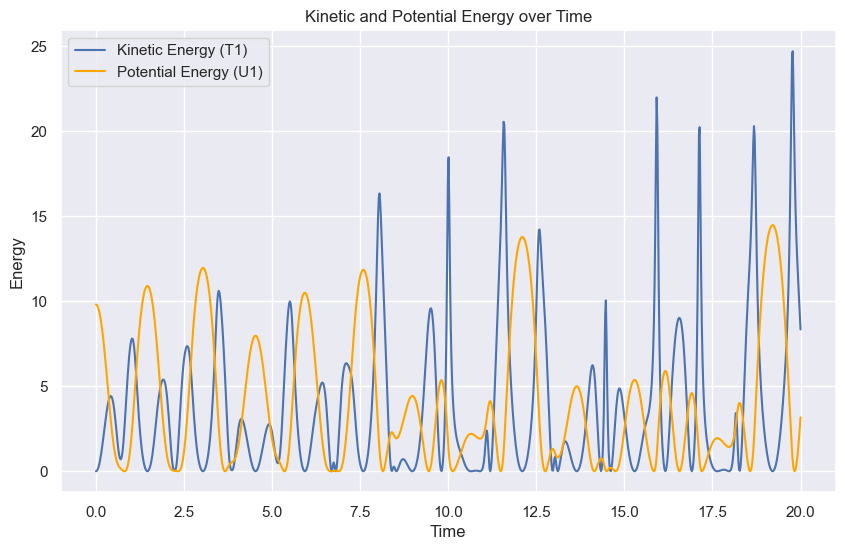
\includegraphics[width=0.8\linewidth]{bob1.png}
    \caption{Change in K.E. and P.E. of bob_{1}\;over time}
\end{figure}
\subsection{Graph of Second Bob}
\begin{figure}[h]
    \centering
    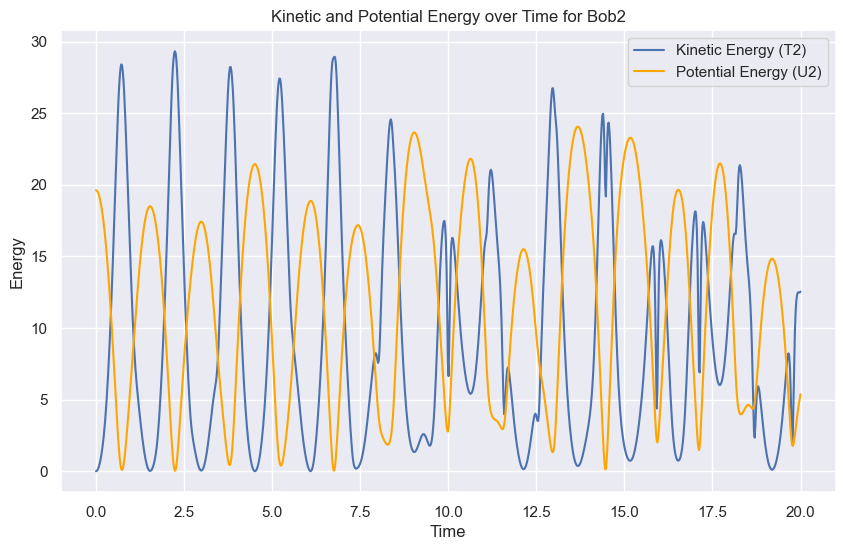
\includegraphics[width=0.8\linewidth]{bob2.png}
    \caption{Change in K.E. and P.E. of bob_{2}\;over time}
\end{figure}

\newpage
\section{Implementation}
Here is a small code snippet of how we can use the equations derived in this document to create a simple simulation of the double pendulum.
\begin{lstlisting}
    import numpy as np
    from scipy.integrate import odeint
    import matplotlib.pyplot as plt
    import matplotlib.animation as animation
    
    g = 9.81
    m1 = 1.0
    m2 = 1.0
    l1 = 1.0
    l2 = 1.0
    
    
    def derivs(state, t):
        theta1, omega1, theta2, omega2 = state
    
        dtheta1dt = omega1
        domega1dt = (
            -g * (2 * m1 + m2) * np.sin(theta1)
            - m2 * g * np.sin(theta1 - 2 * theta2)
            - 2
            * np.sin(theta1 - theta2)
            * m2
            * (l2 * omega2**2 + l1 * omega1**2 * np.cos(theta1 - theta2))
        ) / (l1 * (2 * m1 + m2 - m2 * np.cos(2 * theta1 - 2 * theta2)))
    
        dtheta2dt = omega2
        domega2dt = (
            2
            * np.sin(theta1 - theta2)
            * (
                l1 * (m1 + m2) * omega1**2
                + g * (m1 + m2) * np.cos(theta1)
                + l2 * m2 * omega2**2 * np.cos(theta1 - theta2)
            )
        ) / (l2 * (2 * m1 + m2 - m2 * np.cos(2 * theta1 - 2 * theta2)))
    
        return [dtheta1dt, domega1dt, dtheta2dt, domega2dt]
    
    
    theta1_init = np.pi / 2.0
    omega1_init = 0.0
    theta2_init = np.pi / 2.0
    omega2_init = 0.0
    state_init = [theta1_init, omega1_init, theta2_init, omega2_init]
    
    t = np.linspace(0, 40, 2000)
    
    state = odeint(derivs, state_init, t)
    theta1 = state[:, 0]
    omega1 = state[:, 1]
    theta2 = state[:, 2]
    omega2 = state[:, 3]
    
    x1 = l1 * np.sin(theta1)
    y1 = -l1 * np.cos(theta1)
    x2 = x1 + l2 * np.sin(theta2)
    y2 = y1 - l2 * np.cos(theta2)
\end{lstlisting}
Here, x1, y1 and x2, y2 are positions of the bobs respectively relative to the base of the first rod. You can use these values to generate a simulation of the double pendulum.
\newpage
\section{Conclusion}
The study of the double pendulum system has provided valuable insights into the world of chaotic motion and complex dynamics. Through the application of Lagrangian mechanics, we derived the equations of motion for a double pendulum, demonstrating the system's sensitivity to initial conditions and the resultant unpredictable behavior.
\\\\
By examining the kinetic and potential energies of the system, we were able to express these energies in terms of generalized coordinates, specifically the angles \(\theta_1\) and \(\theta_2\). This approach allowed us to simplify the complex interactions between pendulums and better understand the physics driving the motion.
\\\\
Overall, this project not only deepened our understanding of classical mechanics but also illustrated the profound complexity that can arise even in relatively simple physical systems. The double pendulum serves as a significant example of chaos theory and nonlinear dynamics, providing a compelling case study for both theoretical exploration and practical application in engineering and physics.
\end{document}